\section{Protocolli ausiliari dello strato di rete}

    Per poter spedire i pacchetti su una rete occorre conoscere gli indirizzi fisici dei nodi coinvolti. Un indirizzo fisico è un indirizzo locale (48 bit) che ha significato solo all'interno di una rete. Viene chiamato fisico perché è una proprietà fisica dell'interfaccia di rete.
    
    \vspace{3mm}
    
    Ogni nodo di Internet viene identificato da un indirizzo logico (IP) che identifica il nodo globalmente su Internet e da un indirizzo fisico che identifica il nodo all'interno della rete locale alla quale appartiene.
    
    Ne consegue che la consegna dellle informazioni è su due livelli: logica e fisica. Occorre essere in grado di trasformare un indirizzo logico in fisico (\textit{risoluzione}) e viceversa (\textit{risoluzione inversa}).
    
    Se il client non conosce né il proprio indirizzo IP, né quello di un server centrale, esso può usare tutti 0 come indirizzo sorgente e tutti 1 come indirizzo destinazione. Il messaggio di richiesta verrà spedito in \textbf{broadcast} sulla rete locale. 
    
    \subsection{ARP}
    
        Il protocollo ARP (Address Resolution Protocol) trova l'indirizzo fisico corrispondente ad un indirizzo logico. Tale indirizzo fisico sarà necessario allo strato di collegamento per consegnare un datagram incapsulatoall'interno di un frame; serve, dunque, per la consegna diretta. La risoluzione può essere di due tipi: statica e dinamica.
        
        \vspace{3mm}
        
        La risoluzione statica prevede una tabella delle corrispondenze, nelle quale un indirizzo logico è automaticamente associato ad un indirizzo fisico memorizzato. Lo svantaggio è che questa tabella dev'essere continuamente aggiornata (l'interfaccia di rete può essere cambiata, ad esempio).
        
        \vspace{3mm}
        
        L'ARP prevede una risoluzione dinamica. Il nodo che vuole la traduzione esegue una richiesta ARP, includendo sia il proprio indirizzo IP che l'indirizzo IP da tradurre (cioè quello del destinatario). Questa richiesta è inviata in broadcast sulla rete e ricevuta in unicast.
        
        Usare l'ARP per ogni pacchetto è inefficiente. Se un nodo sorgente deve spedire più pacchetti ad un nodo destinazione, può usare solo una volta il protocollo e memorizzare (in scadenza) i risultati in una cache.
        
        \subsubsection{Formato ARP}
        
            Un messaggio ARP viene incapsulato direttamente in un frame dallo strato di collegamento. La richiesta in sé passa dalo strato di rete allo strato di collegamento, usando l'indirizzo fisico di broadcast come destinazione.
            
            Ogni nodo della rete riceve il frame. Poiché il frame contiene l'indirizzo di broadcast, gli strati di collegamento di tutti i nodi accettano il messaggio e lo passano all'ARP. Solo il protocollo ARP del nodo che ha come indirizzo IP l'indirizzo di destinazione specificato nella richiesta ARP, accetterà il messaggio. Il nodo di destinazione replicherà con una risposta ARP contenenete il suo indirizzo fisico.
            
            Infine, il mittente riceverà una risposta ARP contenente l'indirizzo fisico del destinatario. Adesso, il nodo sorgente può spedire il datagram IP.
            
            \vspace{3mm}
            
            Nel caso di consegne indirette, si risolvono gli indirizzi dei router intermedi fino ad arrivare a destinazione.
        
            \begin{center}
                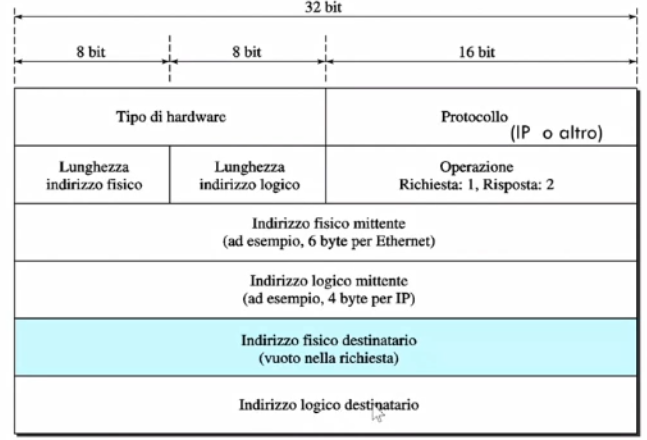
\includegraphics[scale=0.5]{images/ARP.png}
            \end{center}
            
            \begin{itemize}
                \item 
                    \textbf{Hardware (16 bit).} Definisce il tipo di rete che si sta utilizzando. A ogni tipo di rete è associato un codice che ne identifica il tipo. Le reti Ethernet usano il tipo 1.
                
                \item
                   \textbf{ Protocollo (16 bit).} Definisce il tipo di indirizzo logico da gestire (ad esempio l'IPv4).
                
                \item
                   \textbf{ Lunghezza indirizzo fisico (8 bit).} Definisce la lunghezza in byte dell'indirizzo fisico.
                    
                \item
                   \textbf{ Lunghezza indirizzo logico (8 bit).} Definisce la lunghezza in byte dell'indirizzo logico.
                    
                \item
                   \textbf{ Operazione (16 bit).} Definisce il tipo di messaggio ARP. Ne sono previsti due: richiesta ARP (1) e risposta ARP (2).
                    
                \item
                   \textbf{ Indirizzo fisico mittente.} Di lunghezza variabile.
                    
                \item
                   \textbf{ Indirizzo logico mittente.} Di lunghezza variabile.
                    
                \item
                   \textbf{ Indirizzo fisico destinatario.} Di lunghezza variabile. In una richiesta ARP, questo campo è vuoto.
                    
                \item
                   \textbf{ Indirizzo logico destinatario.} Di lunghezza variabile. E' l'indirizzo che si vuole risolvere.
            \end{itemize}
        
            Un \textbf{proxy ARP} gestisce tutte le richieste e risposte ARP per conto dei nodi su una rete. Quando riceve una richiesta ARP, risponderà col proprio indirizzo fisico. In questo modo, sarà il proxy ARP ad inoltrare il datagram IP contenente i dati verso la reale destinazione, una volta risolto l'indirizzo logico.
            
    \subsection{RARP}
    
        Il RARP traduce un indirizzo fisico ad un indirizzo logico. Osserviamo che, in alcuni casi, i computer non conoscono i propri indirizzi logici, ma sicuramente conoscono quello fisico.
        
        Il nodo crea un messaggio di richiesta RARP, inserendo il proprio indirizzo fisico e spedendolo in broadcast sulla rete. Sulla rete sarà presente un nodo (detto \textbf{server RARP}) che, conoscendo tutti gli indirizzi IP associati ad un indirizzo fisico, risponderà con le informazioni richieste.
        
        \vspace{3mm}
        
        RARP è chiaramente inefficiente. Inoltre, non permette al messaggio di andare oltre la rete locale (utilizzando un solo server RARP). Per questo motivo, il protocollo è diventato obsoleto ed è stato sostituito da due nuovi protocolli, BOOTP e DHCP.
        
    \subsection{BOOTP}
    
        Il BOOTP (Boot Protocol) prevede un singolo \textbf{server BOOTP} e un \textbf{relay agent} per ogni rete.
        
        Se il server BOOTP è sulla stessa rete del client, il server riceverà il messaggio e potrà rispondere.
        
        Invece, se non c'è un server BOOTP sulla stessa rete del client, allora il relay agent riceve la richiesta e - conoscendo l'IP del server BOOTP - inoltrerà quest'ultima verso di essa. La risposta del server BOOTP sarà infine spedita al relay agent, che poi inoltrerà a sua volta la risposta al mittente.
        
        Il server BOOTP ha una tabella di associazioni statica, che presenta problemi già noti - motivo per cui è stato introdotto il DHCP.
        
    \subsection{DHCP}
    
        Il DHCP (Dynamic Host Configuration Protocol) risolve il problema dell'assegnazione statica degli indirizzi. Utilizza, infatti, un'assegnazione degli indirizzi IP sia statica che dinamica, permettendo una gestione manuale o automatica del sistema.
        
        L'allocazione dinamica del DHCP prevede che il server DHCP utilizzi un pool di indirizzi liberi che vengono assegnati ad un host che tenta di comunicare. Quando un cliente DHCP richiede l'assegnazione dinamica di un indirizzo IP, il server DHCP consulta il database degli indirizzi dinamici e ne assegna uno all'host (controllando prima la cache e la tabella statica per evitare che si riassegni l'indirizzo). Esiste un meccanismo di \textit{lease} che ordina l'abbondono di un indirizzo IP dinamico dopo un certo periodo di tempo o il rinnovo del lease stesso.
        
    \subsection{ICMP}
    
        L'ICMP (Internet Control Message Protocol) notifica situazioni di errore e permette di inviare messaggi di richiesta.
        
        I messaggi di notifica degli errori consistono in segnalazioni di eventuali problemi che un router o la destinazione finale hanno riscontrato durante la gestione di un pacchetto.
        
        I messaggi di richiesta permettono ad un host di ottenere informazioni specifiche da altri nodi della rete (riguardanti i nodi ad esso direttamente connessi, ad esempio). I router possono fornire informazioni adli host per spedire i pacchetti IP su percorsi più efficienti.
        
        \vspace{3mm}
        
        Il formato di un messaggio ICMP prevede:
        
        \begin{itemize}
            \item 
                \textbf{Tipo (8 bit).} Specifica il tipo di messaggio ICMP. Ad esempio:
                    \begin{itemize}
                        \item 
                            3. Destinazione non raggiungibile (l'applicazione a livello superiore non esiste; il datagram non può essere consegnato)
                            
                        \item 
                            4. Rallentamento sorgente (router congestionato; buffer pieno)
                            
                        \item 
                            11. Tempo scaduto (TTL a 0)
                            
                        \item 
                            12. Problemi con i parametri (qualsiasi ambiguità nell'intestazione)
                            
                        \item 
                            5. Ridirezione (un router si accorge che la sorgente dovrebbe spedire il datagram verso un altro router)
                            
                        \item
                            8 e 0. Richiesta e risposta \textit{echo}. Usato per diagnosticare problemi della rete, e cioè per vedere se un nodo risponde ("\textit{ping}").
                        
                        \item 
                            13 e 14. Richiesta e risposta \textit{timestamp}. Usato per controllare il tempo di andata e ritorno necessario ad un datagram per viaggiare fra due nodi.
                            
                        \item
                            17 e 18. Richiesta e risposta maschera di rete. Usati per controllare la maschera di sottorete.
                            
                        \item
                            10 e 9. Sollito e presenza router. Usati per ottenere l'indirizzo IP di un router.
                    \end{itemize}
            
            \item 
                \textbf{Codice (8 bit).} Specifica la motivazione che ha portato alla creazione del messaggio.
                
            \item
                \textbf{Somma di controllo.} Campo di rilevazione degli errori.
                
            \item
                \textbf{Dati.} Riporta informazioni che permettono di individuare il pacchetto per il quale si è verificato l'errore (se il messaggio è di tipo di notifica degli errori), e cioè i primi 8 byte del datagram che corrispondono all'indirizzo IP, o altre informazioni che dipendono dal tipo di richiesta.

        \end{itemize}
        
        \subsubsection{Ping e Traceroute}
        
            Il comando \textbf{ping} utilizza i messaggi ICMP di richiesta e risposta echoi per stabilire se un host è attivo e risponde. L'host mittente spedisce un messaggio ICMP di richiesta echo; la destinazione, se attiva, risponderà con un messaggio ICMP di risposta echo. Il comando ping spedisce continuamente, finché non viene interrotto. Inoltre, viene calcolato il tempo di andata e ritorno per ogni coppia di richiesta e risposta echo.
        
            \vspace{3mm}
        
            Il comando \textbf{traceroute} scopre la sequenza di router che attraverserebbe un datagram IP dalla sorgente alla destinazione, delineando quindi una rotta. Sfrutta i messaggi ICMP (tempo scaduto e messaggio di destinazione non raggiungibile) e si trova nello strato di applicazione ed usa UDP come protocollo.
            
            Un pacchetto vuole viaggiare da un nodo A al nodo B, e per farlo deve attraverssare due router $R_1$ e $R_2$. Il programma traceroute sul nodo A spedisce un pacchetto alla destinazione B usando il protocollo UDP. Il messaggio viene incapsulato in un pacchetto IP ed il valore TTL viene impostato a 1. Il router R1 riceve il pacchetto e decrementa il TTL che diventa 0; il router, quindi, scarterà il pacchetto e invierà un messaggio ICMP di tempo scaduto alla sorgente. 
            
            Il nodo sorgente A riceverà il messaggio che, ovviamente, conterrà l'indirizzo logico del router, scoprendo quindi il primo router nel percorso verso il nodo destinazione, salvandosi anche il tempo di invio dela richiesta. Il prossimo step sarà inviare un traceroute con TTL a 2, in modo da superare il router già visitato. Il procedimento se itera fino al raggiungimento del nodo di destinazione.
        
            \vspace{3mm}
        
            Per ricevere un messaggio di errore, traceroute usa una strategia diversa. La porta di destinazione del pacchetto UDP viene posta a 1 (che non è un valore supportato). Quando l'host B riceve il pacchetto UDP, non riuscirà a trovare un'applicazione che accetti la porta. Pertanto il pacchetto verrà eliminato e un messaggio ICMP di destinazione non raggiungibile sarà spedito al nodo A.
            
            La ricezione di un messaggio di errore ICMP di destinazione non raggiungibile indica anche che il percorso è stato scoperto completamente e quindi che il programma traceroute può terminare la propria esecuzione.